\documentclass{scrartcl}

% packages
\usepackage{amsmath}
\usepackage{amssymb}
\usepackage[ngerman]{babel}
\usepackage{booktabs}
\usepackage[font=small,labelfont=bf]{caption}
\usepackage{csquotes}
\usepackage{float}
\usepackage{fontspec}
  \setmainfont[Ligatures=TeX]{Tex Gyre Pagella}
\usepackage{graphicx}
\usepackage[pdfusetitle,unicode]{hyperref}
\usepackage{mathtools}
\usepackage{microtype}
\usepackage{siunitx}
  \sisetup{separate-uncertainty=true}
\usepackage{subcaption}
\usepackage[math-style=ISO,bold-style=ISO]{unicode-math}
  \setmathfont{Tex Gyre Pagella Math}
\usepackage{xfrac}

% options
\setlength{\parindent}{0pt}  % no stupid indentation

% commands
\DeclarePairedDelimiter{\abs}{\lvert}{\rvert}
\DeclarePairedDelimiter{\mean}{\langle}{\rangle}
\renewcommand{\vec}[1]{\mathbf{#1}}
\renewcommand{\i}{\mathrm{i}}
\DeclareRobustCommand{\e}{\ensuremath{\mathrm{e}}}

% meta
\author{Kevin Dungs \and Kevin Heinicke \and Holger Stevens}
\title{Computational Physics}
\subtitle{Übungsblatt 6}

% document
\begin{document}
\maketitle

\section*{Hausaufgabe 12: MC Simulation des 2-D Ising-Modells (Teil 2)}

\paragraph{(a)} In \autoref{fig:crit} bestätigt sich die Abschätzung
\begin{equation}
  T_c = \frac{2}{\ln\left(1 + \sqrt{2}\right)}
\end{equation}

\begin{figure}[H]
    \centering
    \begin{subfigure}{.48\textwidth}
      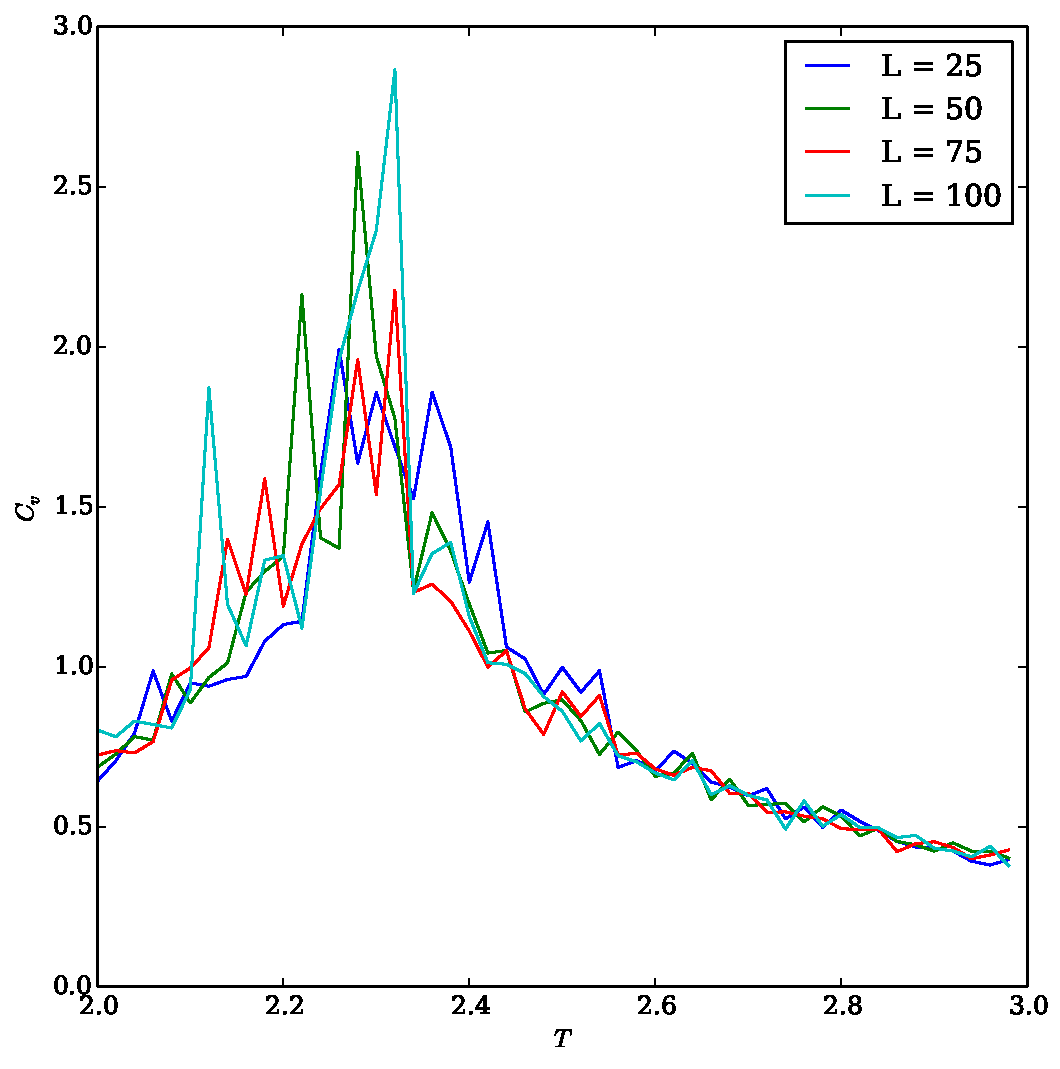
\includegraphics[width=\textwidth]{plots/crit.pdf}
      \caption{Verlauf der spezifischen Wärmekapazität in Abhängigkeit der Temperatur.}
    \end{subfigure} %
    \begin{subfigure}{.48\textwidth}
      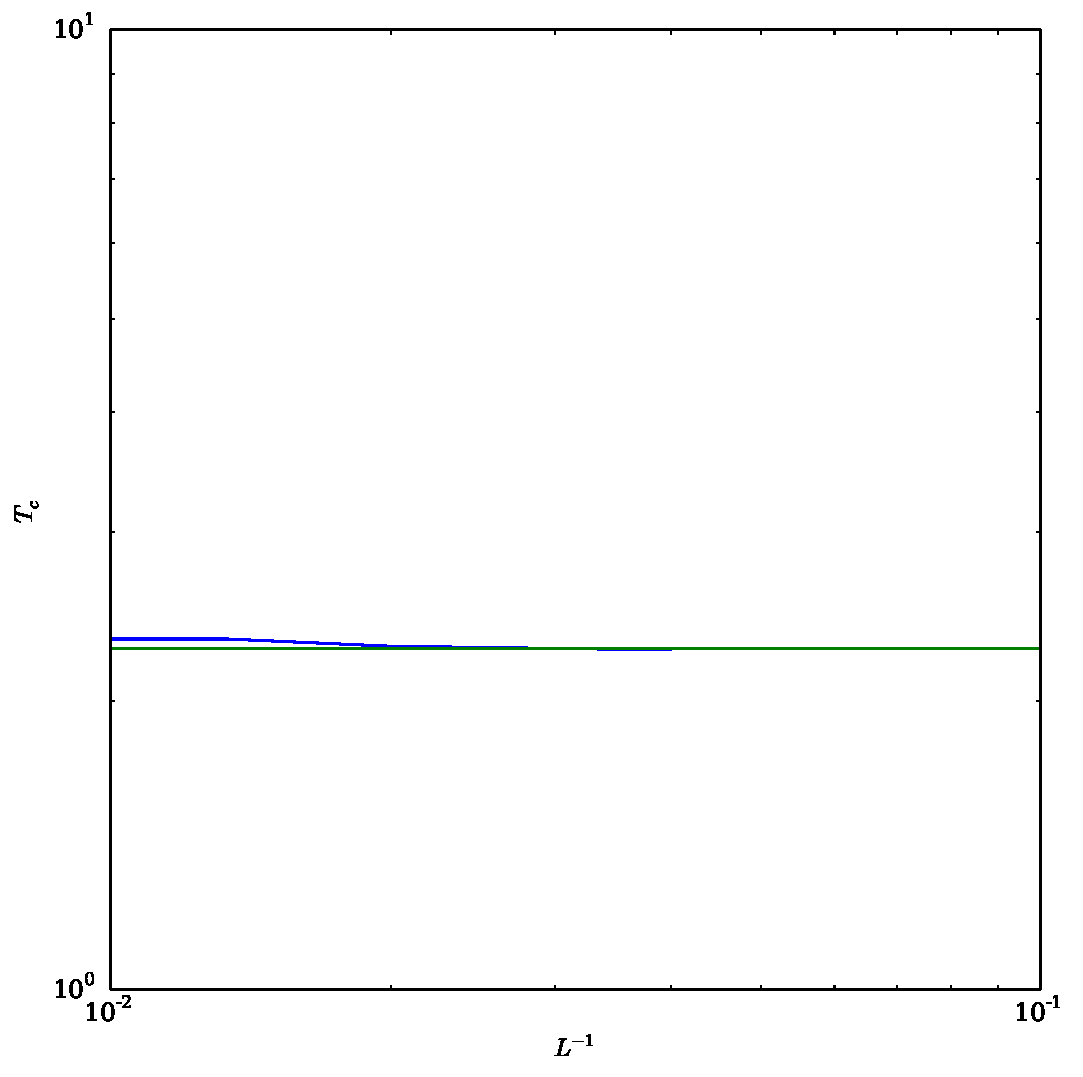
\includegraphics[width=\textwidth]{plots/Tc_L.pdf}
      \caption{Doppeltlogarithmischer Plot der kritischen Temperatur gegen die inverse Systemgröße.}
    \end{subfigure}
    \caption{}
    \label{fig:crit}
\end{figure}


\paragraph{(b)} In \autoref{fig:magnetisation} ist der Verlauf der Magnetisierung für verschiedene Systemgrößen und Temperaturen aufgetragen. Es ist zu sehen, dass die Kurven bei $T = T_c$ kollabieren.

\begin{figure}[H]
    \centering
    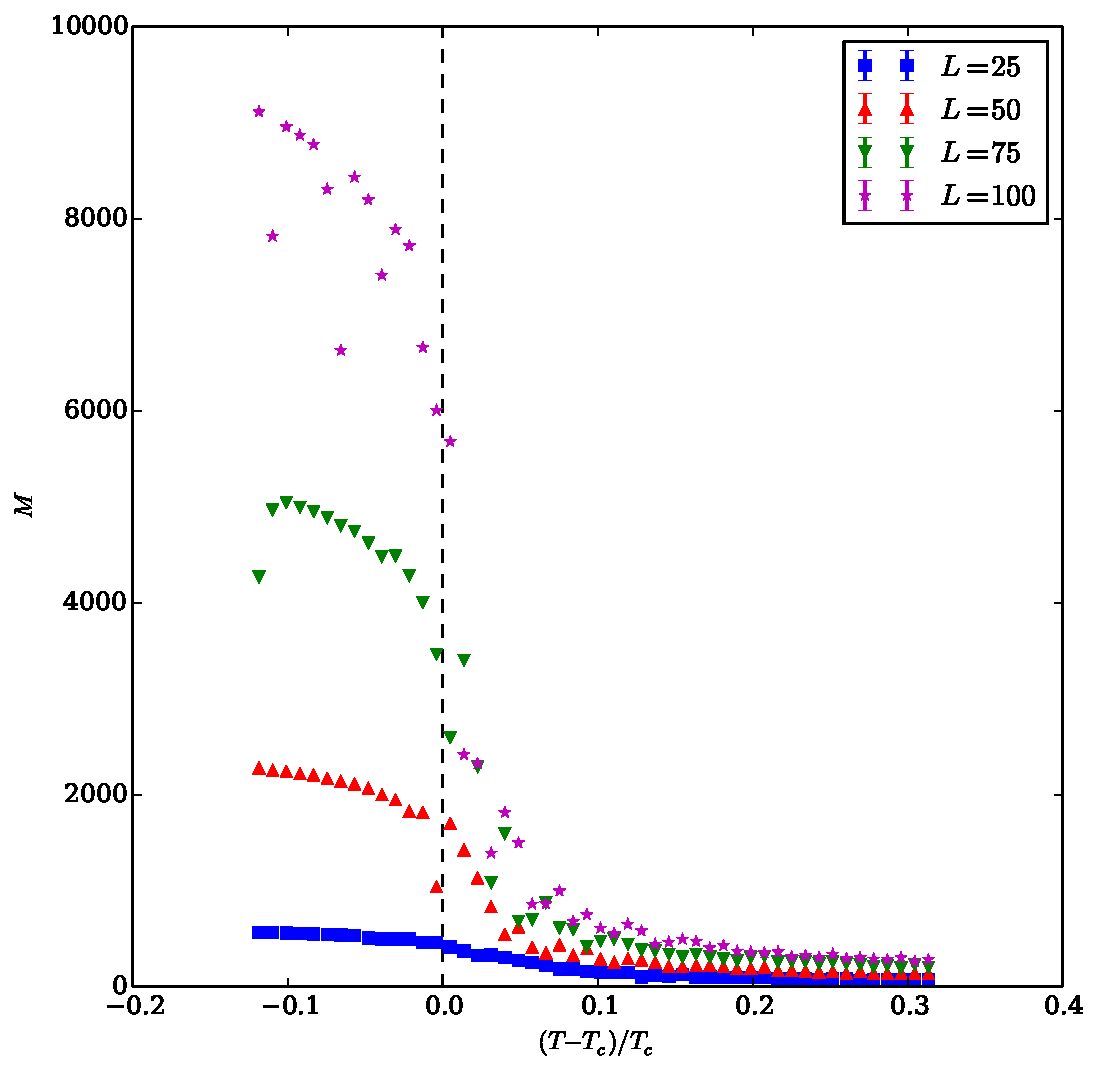
\includegraphics[width=.5\textwidth]{plots/magnetisation.pdf}
    \caption{Verlauf der spezifischen Wärmekapazität in Abhängigkeit der Temperatur.}
    \label{fig:magnetisation}
\end{figure}


\paragraph{(c)} Wir lassen uns einfach die Varianz ebenso berechnen, wie den Mittelwert. Dann brauchen wir keine Samples zu speichern und kein Bootstrapping zu betreiben. Dazu musste das Programm lediglich dahingehend verändert werden, dass der \texttt{MagnetisationCalculator} auch noch den Fehler auf den Mittelwert bzw. die Varianz aus \texttt{RunningStats} zurück gibt.

\end{document}
